\documentclass[11pt]{article}


\setlength{\oddsidemargin}{-0.25 in}
\setlength{\evensidemargin}{-0.25 in}
\setlength{\topmargin}{-0.9 in}
\setlength{\textwidth}{7.0 in}
\setlength{\textheight}{9.0 in}
\setlength{\headsep}{0.75 in}
\setlength{\parindent}{0.3 in}
\setlength{\parskip}{0.1 in}
\usepackage{epsf}
\usepackage{pseudocode}
\usepackage{dsfont}
\usepackage{amssymb}
\usepackage{amsmath}
\usepackage{graphicx}


\begin{document}
\title{Programming Assignment 2}
\author{Aron Szanto\\
 Artidoro Pagnoni}
\date{\today}
\maketitle


\section*{Title of our section}

\begin{center}
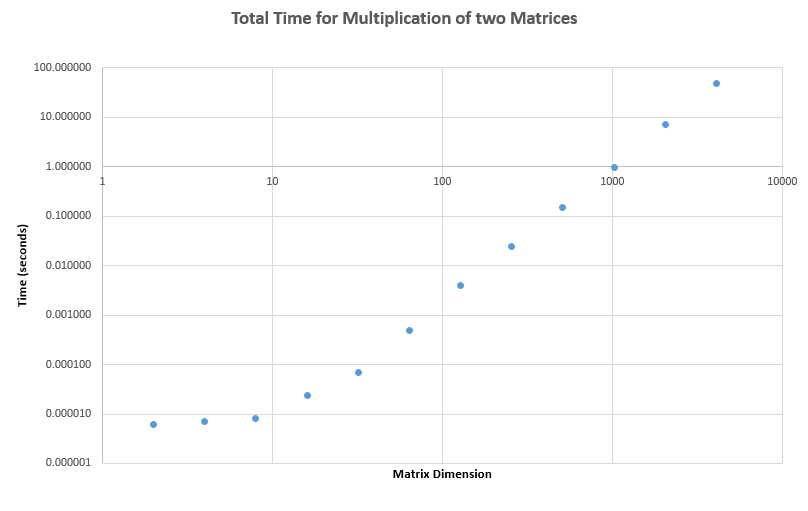
\includegraphics[scale=0.8]{totaltime}
\end{center}


\begin{center}
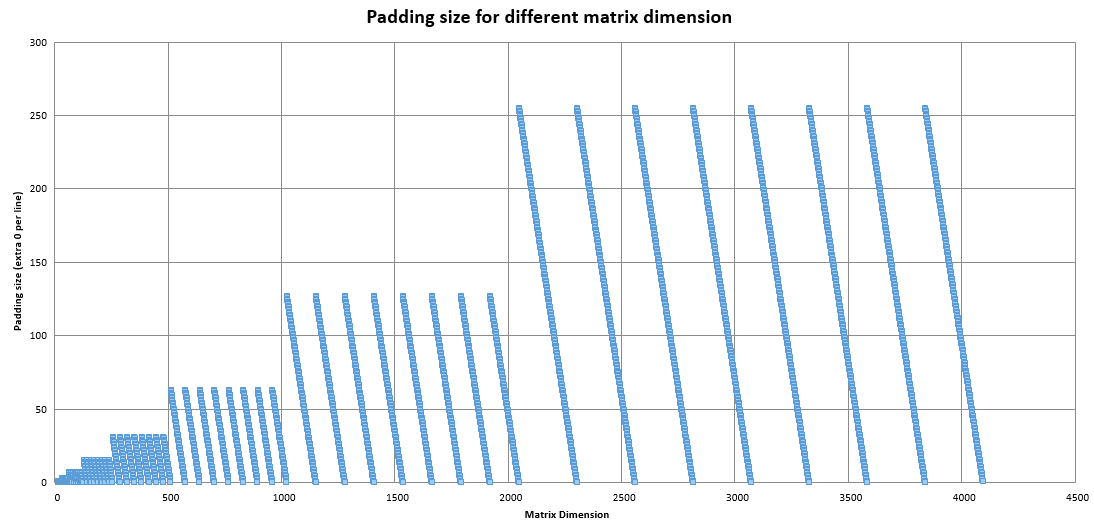
\includegraphics[scale=0.65]{paddingsize}
\end{center}


\begin{center}
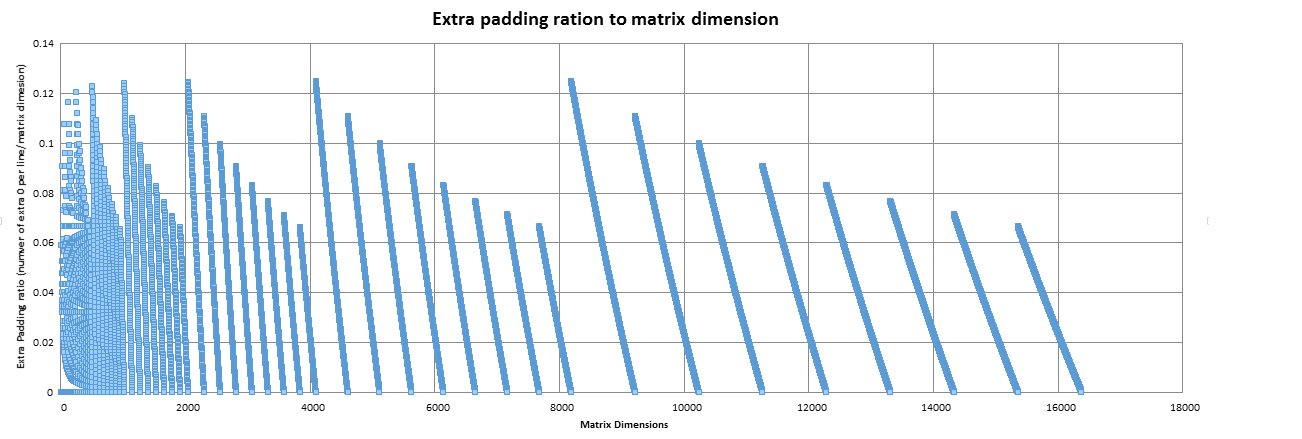
\includegraphics[scale=0.6]{padddingration}
\end{center}


\begin{center}
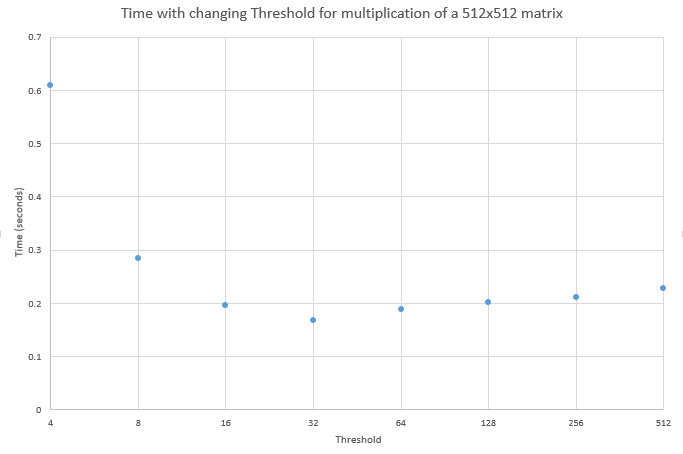
\includegraphics[scale=0.9]{threshold512}
\end{center}


\begin{center}
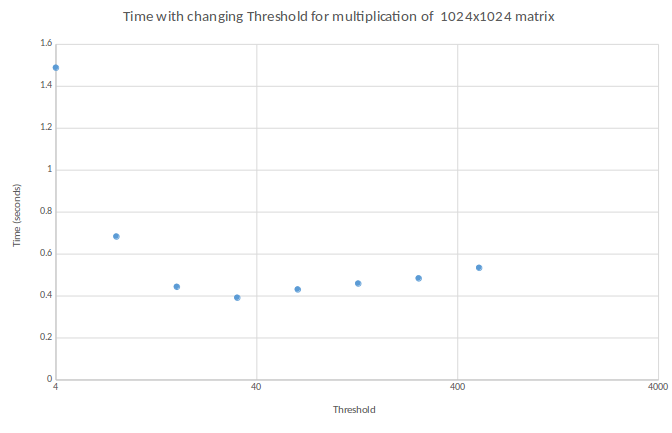
\includegraphics[scale=0.9]{threshold1024}
\end{center}


\begin{center}
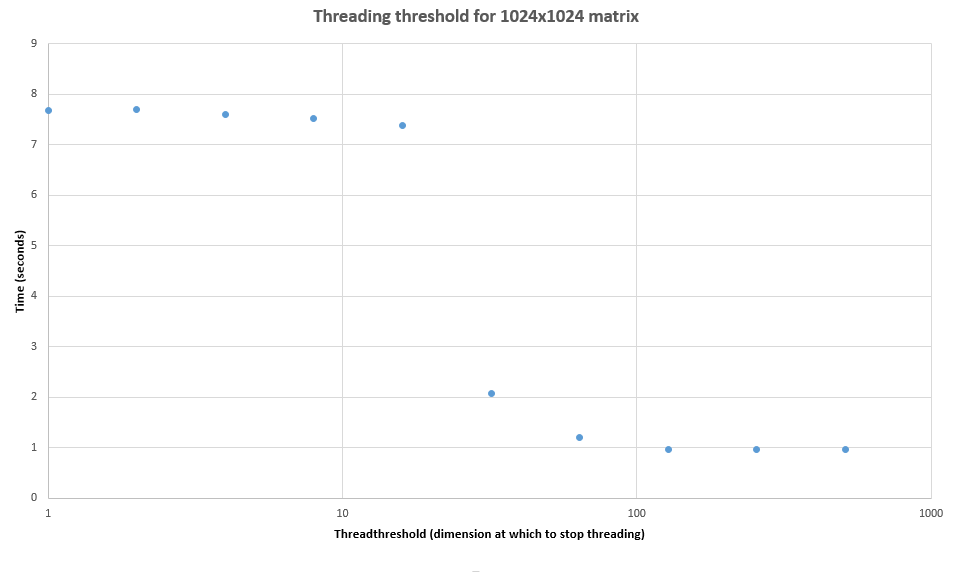
\includegraphics[scale=0.7]{threadthreashold}
\end{center}
















\end{document}



